\section{Поиск критической точки модели IsingISAW на треугольной решётке}

В данном разделе проводится исследование критической области модели Изинга на случайном блуждания без самопересечений (далее, IsingISAW) на треугольной решётке.
В отличие от классической модели на квадратной решётке, узлы треугольной решётки имеют две дополнительные связи по одной из диагоналей (см. рисунок \ref{fig:lattices}), 
вследствие чего координационное число данной модификации (кол-во возможных связей у одного узла) увеличено по сравнению с квадратной с 4 до 6.

Были проведены симуляции Монте-Карло при нулевом внешнем поле и $J \in [0,0.9]$. 
Итоговое количество шагов симуляций от $10^10$ до $10^11$, симулированные блуждания имеют длину $N$ от 100 до 7200.
Были собраны данные для удельной энергии системы на спин $\la \epsilon \ra$ и средняя 2-я и 4-я степени намагниченности на спин $\la m^2 \ra$, $\la m^4 \ra$.
Так же собрана статистика среднего расстояния между концами блуждания $R^2_N$.

\begin{figure}[h]
\centering
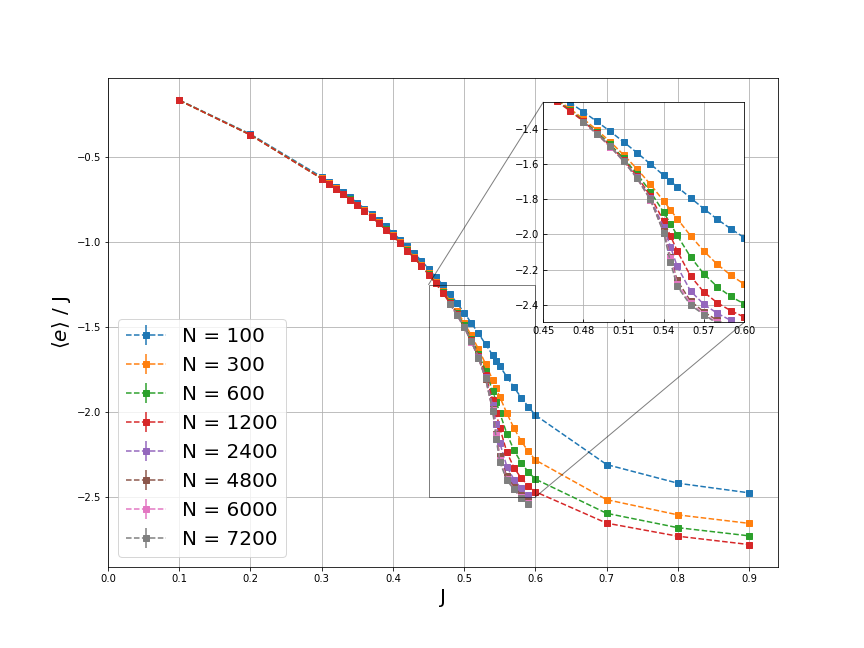
\includegraphics[width=0.7\textwidth]{IsISAW_E.png}
\caption{Удельная энергия узла модели IsingISAW (без учёта константы $J$), с длиной конформации от 100 до 7200 (длины отмечены разными цветами)}
\label{fig:TrIsISAW_E}
\end{figure}

На графике \ref{fig:TrIsISAW_E} показана зависимость удельной энергии узла IsingISAW на треугольной решётке.
График показывает что удельная энергия системы стремится к -3J в пределе бесконечной длины конформации, 
что логично, поскольку с ростом $J$ узлы приобретают наиболее возможное число связей (то есть, 6), но так как связи существуют между парами узлов,
необходимо поделить число связей на 2.
При малых $J$ энергия почти не зависит от длины цепочки $N$, но начиная с $J > 0.53$, расхождение графиков становится наиболее четким.

\begin{figure}[h]
\centering
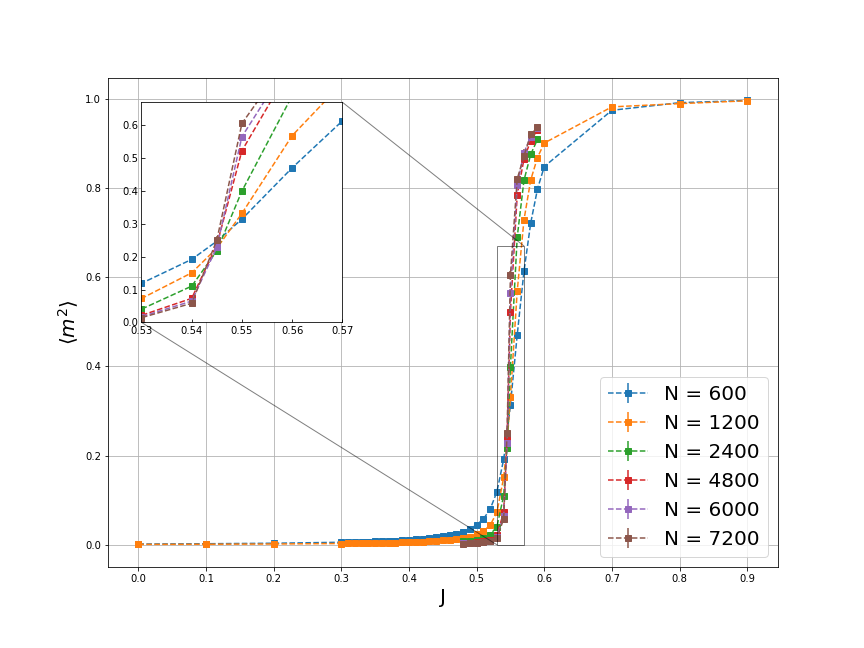
\includegraphics[width=0.7\textwidth]{IsISAW_m2.png}
\caption{Средняя вторая степень намагниченности узла модели IsingISAW с длиной конформации от 100 до 7200 (длины отмечены разными цветами)}
\label{fig:TrIsISAW_m2}
\end{figure}

На графике \ref{fig:TrIsISAW_E} изображен момент намагниченности второго порядка в зависимости от $J$.
Пересечение графиков величины для конформаций разных длин имеют четкое пересечение в $J \approx 0.545$.

